\chapter{Voronoi Diagrams}
\label{ch:voronoi_diagrams}

\section{Voronoi Diagram}
\label{sec:voronoi_diagram}

A Voronoi diagram\index{Voronoi diagram} partitions the plane into regions
based on distance to a set of sites. The cell of a site contains the points
closer to it than to any other site. The Voronoi diagram is the geometric dual
of the Delaunay triangulation~\cite{voronoi1908,aurenhammer1991}.

\subsection{Definitions}

\begin{definition}[Voronoi Cell]\label{def:voronoi_cell}
For sites $S = \{s_1,\ldots,s_n\} \subset \mathbb{R}^2$, the Voronoi cell of $s_i$
is
\[
V(s_i) = \{p \in \mathbb{R}^2 \mid \|p-s_i\| \leq \|p-s_j\|\text{ for all }j\ne i\}.
\]
\end{definition}

\begin{definition}[Voronoi Vertex]\label{def:voronoi_vertex}
A Voronoi vertex is a point where three or more cells meet. It is equidistant
from its closest sites and corresponds to the circumcenter of a Delaunay
triangle.
\end{definition}

\subsection{Delaunay Duality}

The duality is given by the following correspondences:
\begin{enumerate}
\item A Delaunay vertex corresponds to a Voronoi cell.
\item A Delaunay triangle corresponds to a Voronoi vertex.
\item A Delaunay edge corresponds to a Voronoi edge on a perpendicular bisector.
\end{enumerate}

\begin{theorem}[Duality of Delaunay and Voronoi Diagrams]\label{thm:dt_vd_duality}
For sites in general position, the Delaunay triangulation and Voronoi diagram
are planar duals and both have linear complexity.
\end{theorem}

\begin{figure}[htbp]
\centering
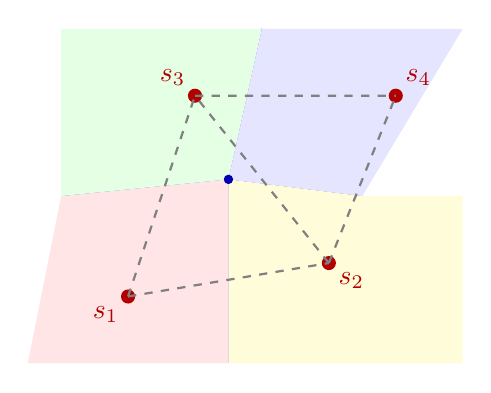
\begin{tikzpicture}[scale=0.85]
  \coordinate (s1) at (0,0);
  \coordinate (s2) at (3,0.5);
  \coordinate (s3) at (1,3);
  \coordinate (s4) at (4,3);
  \draw[blue!60,thick] (-1,1.5)--(1.5,1.75)--(3.5,1.5);
  \draw[blue!60,thick] (1.5,1.75)--(2,4);
  \draw[blue!60,thick] (1.5,1.75)--(1.5,-1);
  \fill[red!10] (-1.5,-1)--(-1,1.5)--(1.5,1.75)--(1.5,-1)--cycle;
  \fill[green!10] (1.5,1.75)--(-1,1.5)--(-1,4)--(2,4)--cycle;
  \fill[blue!10] (1.5,1.75)--(2,4)--(5,4)--(3.5,1.5)--cycle;
  \fill[yellow!15] (1.5,1.75)--(3.5,1.5)--(5,1.5)--(5,-1)--(1.5,-1)--cycle;
  \fill[red!70!black] (s1) circle (3pt) node[below left] {$s_1$};
  \fill[red!70!black] (s2) circle (3pt) node[below right] {$s_2$};
  \fill[red!70!black] (s3) circle (3pt) node[above left] {$s_3$};
  \fill[red!70!black] (s4) circle (3pt) node[above right] {$s_4$};
  \draw[gray,dashed,thick] (s1)--(s2) (s1)--(s3) (s2)--(s3) (s2)--(s4) (s3)--(s4);
  \fill[blue!70!black] (1.5,1.75) circle (2pt);
\end{tikzpicture}
\caption{Voronoi diagram (colored cells) and its Delaunay triangulation dual (dashed gray edges). Each Voronoi vertex is the circumcenter of a Delaunay triangle.}
\label{fig:voronoi_duality}
\end{figure}


\subsection{Pseudocode}

\begin{algorithm}[htbp]
\caption{Voronoi Diagram via Delaunay Dual}
\label{alg:voronoi}
\begin{algorithmic}[1]
\Function{ComputeVoronoi}{sites, bounding\_box}
  \State $DT \gets \text{DelaunayTriangulation}(sites)$
  \State $C \gets \{\text{Circumcenter}(T) : T \in DT.triangles\}$
  \For{$site$ in $sites$}
    \State $star \gets \text{FindTrianglesSharingVertex}(site, DT)$
    \State $boundary \gets \text{SortAround}(site, C[star])$
    \State $cell \gets \text{ClipPolygon}(boundary, bounding\_box)$
    \State Store $cell$
  \EndFor
  \State \Return all stored cells
\EndFunction
\end{algorithmic}
\end{algorithm}

\subsection{Complexity and Applications}

Construction through a Delaunay triangulation takes $O(n\log n)$ time and
$O(n)$ space. A bounding box is required to cap cells belonging to sites on
the convex hull. Applications include facility location, robot path planning,
territory modeling, and nearest-neighbor search.

\subsection{Testing and Edge Cases}

Sites on the convex hull produce unbounded cells, co-circular sites produce
non-unique vertices, collinear sites create degeneracies, and duplicate sites
must be merged or rejected.

\section{Voronoi Diagrams of Line Segments}
\label{sec:voronoi_segments}

The generalized Voronoi diagram of a set of disjoint line segments
$S = \{s_1, \dots, s_n\}$ partitions the plane according to the Euclidean
distance to the closest point of each segment. Segment sites arise whenever
features are modeled as one-dimensional objects: road networks, rivers, and
walls in GIS, or the edges of polygonal obstacles in robot motion
planning~\cite{leedrysdale1981,okabe2000}. The medial axis of a polygonal
domain is a subset of this diagram.

\subsection{Definitions}

\begin{definition}[Distance to a Segment]\label{def:distance_to_segment}
The distance from a point $p$ to a closed segment $s = \overline{ab}$ is
\[
\operatorname{dist}(p, s) = \min_{q \in s} \|p - q\|_2,
\]
attained at the orthogonal projection of $p$ onto the supporting line of $s$
clamped to $[a, b]$; if the projection falls outside the segment, the minimum
is attained at the nearer endpoint.
\end{definition}

\begin{definition}[Voronoi Cell of a Segment]\label{def:segment_voronoi_cell}
The Voronoi cell of segment $s_i$ is
\[
V(s_i) = \{p \in \mathbb{R}^2 \mid \operatorname{dist}(p, s_i) \le \operatorname{dist}(p, s_j)\text{ for all } j \ne i\}.
\]
\end{definition}

\subsection{Theory}

The bisector of two sites is the locus of points equidistant from them. For
segment sites the bisector is composed of
\begin{itemize}
\item a \textbf{line} between two points (or between two parallel segment
  interiors),
\item a \textbf{parabola} whose focus is a segment endpoint and whose
  directrix is the supporting line of the other segment, or
\item an \textbf{angle bisector} between two non-parallel supporting lines.
\end{itemize}

Consequently the edges of a segment-site Voronoi diagram are straight segments
or parabolic arcs, and its cells are star-shaped but not necessarily convex.

\begin{theorem}[Complexity of the Segment Voronoi Diagram]\label{thm:segment_voronoi_complexity}
The Voronoi diagram of $n$ disjoint line segments has $O(n)$ vertices, edges,
and cells, and can be computed in $O(n \log n)$ time.
\end{theorem}
\begin{proof}[Proof sketch]
Each segment contributes a bounded number of features, and the planar
structure of the diagram bounds the total complexity linearly. The $O(n \log
n)$ construction time is achieved by Fortune's sweep-line algorithm
generalized to segment sites---the beach line then alternates between parabolic
arcs (foci at segment endpoints) and line segments---and by divide-and-conquer
constructions~\cite{fortune1987,leedrysdale1981}.
\end{proof}

\subsection{Pseudocode}

\begin{algorithm}[htbp]
\caption{Segment Voronoi Diagram by Plane Sweep}
\label{alg:segment_voronoi}
\begin{algorithmic}[1]
\Function{SegmentVoronoi}{segments}
  \State $Q \gets$ site events (segment endpoints) and circle events
  \State $T \gets$ balanced tree holding the beach line of lines and parabolas
  \State initialize output structure for each segment
  \While{$Q$ is not empty}
    \State $e \gets Q.\text{pop}()$
    \If{$e$ is a site event}
      \State insert the new beach-line arc into $T$
      \State detect and schedule new circle events
    \Else \Comment{circle event: an arc disappears}
      \State create a Voronoi vertex and its incident edges
      \State remove the arc and update circle events
    \EndIf
  \EndWhile
  \State \Return edges and vertices, clipped to the bounding box
\EndFunction
\end{algorithmic}
\end{algorithm}

\subsection{Complexity and Applications}

The diagram needs $O(n \log n)$ time and $O(n)$ space. Applications include
\begin{itemize}
\item the \textbf{medial axis} of a polygonal domain (a subset of the
  diagram),
\item \textbf{nearest-obstacle} and clearance queries for a robot among
  polygonal obstacles, and
\item \textbf{1-skeleton} neighborhood queries in road and river networks.
\end{itemize}

\subsection{Testing and Edge Cases}

Collinear overlapping segments, parallel segments (whose bisectors are
parallel lines), shared endpoints, and segments touching the bounding box must
be handled; predicates for parabolic bisectors need care near focus
degeneracies.

\section{Farthest-Point Voronoi Diagrams}
\label{sec:farthest_point_voronoi}

The farthest-point Voronoi diagram\index{farthest-point Voronoi diagram}
assigns to each site the region of points for which that site is the
\emph{farthest} among all sites. It is the exact analogue of the ordinary
Voronoi diagram with $\min$ replaced by $\max$, and it is the key structure for
computing the diameter and the smallest enclosing circle of a point
set~\cite{shamos1975,okabe2000}.

\subsection{Definitions}

\begin{definition}[Farthest-Point Voronoi Cell]\label{def:farthest_voronoi_cell}
For sites $S = \{s_1, \dots, s_n\} \subset \mathbb{R}^2$, the farthest-point
Voronoi cell of $s_i$ is
\[
V^\star(s_i) = \{p \in \mathbb{R}^2 \mid \|p - s_i\| \ge \|p - s_j\|\text{ for all } j \ne i\}.
\]
\end{definition}

\subsection{Theory}

\begin{theorem}[Structure of the Farthest-Point Voronoi Diagram]\label{thm:farthest_voronoi_structure}
A site has a non-empty farthest-point Voronoi cell if and only if it is a
vertex of the convex hull of $S$. If the hull $\mathcal{H}(S)$ has $m$
vertices, the farthest-point Voronoi diagram has $m$ cells and $m - 2$
vertices, is a tree, and its edges lie on perpendicular bisectors of pairs of
hull vertices.
\end{theorem}

The diagram is the dual of the Delaunay triangulation of the hull vertices
restricted to the upper side of the lifted paraboloid: a farthest-point
Voronoi vertex is the center of a circle through three hull vertices that
contains all of $S$. Both the nearest- and farthest-point diagrams can be
obtained from the same sweep-line construction by duality~\cite{fortune1987}.

\subsection{Applications: Diameter and Smallest Enclosing Circle}

The principal use of the farthest-point Voronoi diagram is optimization over
the point set:
\begin{itemize}
\item \textbf{Diameter}: the two points realizing the diameter of $S$ are the
  endpoints of an edge of the farthest-point Delaunay diagram of the hull; the
  diameter is found in $O(n \log n)$ time by rotating calipers on the hull.
\item \textbf{Smallest enclosing circle}: the center of the minimum-radius
  circle enclosing $S$ is either a farthest-point Voronoi vertex (the center
  of a circle through three hull vertices that contains all points) or the
  midpoint of a diameter pair. Welzl's randomized algorithm
  \cite{welzl1991} solves the same problem directly in expected linear time.
\end{itemize}

\subsection{Pseudocode}

\begin{algorithm}[htbp]
\caption{Smallest Enclosing Circle via Farthest-Point Voronoi}
\label{alg:farthest_enclosing_circle}
\begin{algorithmic}[1]
\Function{SmallestEnclosingCircle}{points}
  \State $H \gets \text{ConvexHull}(points)$
  \State $FPV \gets \text{FarthestPointVoronoi}(H)$
  \State $best \gets$ circle through the two points of the diameter of $H$
  \For{vertex $v$ of $FPV$}
    \State $C \gets$ circle centered at $v$ through its three hull vertices
    \If{radius$(C) < $ radius$(best)$ and $C$ encloses all points}
      \State $best \gets C$
    \EndIf
  \EndFor
  \State \Return $best$
\EndFunction
\end{algorithmic}
\end{algorithm}

\subsection{Complexity and Applications}

The hull takes $O(n \log n)$ time; the farthest-point Voronoi diagram of the
$m$ hull vertices is a tree with $m$ cells and takes $O(m)$ time and space
once the hull is known. Scanning its vertices costs $O(m)$, for an overall
$O(n \log n)$.

\subsection{Testing and Edge Cases}

Collinear point sets (the diagram degenerates to parallel slabs), co-circular
hull vertices, and hulls with very few vertices (with two points every cell is
a half-plane) are the main edge cases.

\subsection{References}

\begin{itemize}
\item Shamos, M.~I. (1978). ``Computational Geometry''. PhD thesis, Yale
  University.
\item Fortune, S. (1987). ``A sweepline algorithm for Voronoi diagrams.'' 
\item Okabe, A., Boots, B., Sugihara, K., \& Chiu, S.~N. (2000). ``Spatial
  Tessellations: Concepts and Applications of Voronoi Diagrams''. Wiley.
\end{itemize}

\section{Kinetic Voronoi Diagrams}
\label{sec:kinetic_voronoi}

A kinetic Voronoi diagram maintains the diagram of moving sites. Its dual is
maintained through a kinetic Delaunay triangulation. Certificates based on the
in-circle predicate predict when an edge becomes invalid; the next event is
then processed by an edge flip.

\begin{algorithm}[htbp]
\caption{Kinetic Voronoi Maintenance}
\label{alg:kinetic_voronoi}
\begin{algorithmic}[1]
\Function{MaintainKineticVoronoi}{points, trajectories}
  \State $DT \gets \text{DelaunayTriangulation}(points)$
  \State $Q \gets \text{PriorityQueueOfCertificateFailures}(DT, trajectories)$
  \While{$Q$ is not empty}
    \State $event \gets Q.\text{pop}()$
    \State Flip the invalid edge in $DT$
    \State Update certificates for affected edges
  \EndWhile
\EndFunction
\end{algorithmic}
\end{algorithm}

The event-driven structure processes $O(\log n)$ priority-queue work per
event. Degenerate cases include zero-velocity sites, collisions, simultaneous
co-circular events, and sites leaving the region of interest.

\begin{itemize}
\item Voronoi, G. (1908). ``Nouvelles applications des param\`etres continus.''
\item Fortune, S. (1987). ``A sweepline algorithm for Voronoi diagrams.''
\item Aurenhammer, F. (1991). ``Voronoi Diagrams: A Survey.''
\end{itemize}

\section{Industrial Applications of Voronoi Diagrams}
\label{sec:voronoi_applications}

Voronoi diagrams appear throughout industry because the dual Delaunay
triangulation (Section~\ref{sec:delaunay_duality}) and the nearest-site
assignment they encode are the exact solution to many ``assign each point to
the closest resource'' problems. The following are the principal industrial
use cases.

\begin{itemize}
\item \textbf{Retail and Service-Area Analysis (GIS)}: Retail chains, banks,
  and emergency services use the Voronoi diagram (``Thiessen polygons'') of
  existing sites to compute service territories and to find the location of a
  new facility that maximizes the underserved area---the site whose insertion
  grows the smallest uncovered Voronoi cell the most. Thiessen-polygon
  generation is a standard tool in commercial GIS---\texttt{Esri ArcGIS}
  (3D Analyst) and MapInfo---sold to thousands of planning
  departments~\cite{okabe2000}.

\item \textbf{Wireless and Cellular Network Planning}: The Voronoi cells of
  base stations or small cells are the coverage regions under nearest-site
  association; load balancing and cell planning are performed directly on
  these cells, and the Delaunay graph gives the interference and handover
  topology. Commercial RF-planning suites (Atoll, Planet) sold to carriers
  and network operators build on this decomposition~\cite{okabe2000}.

\item \textbf{Logistics and Field-Service Territory Design}: Voronoi
  territories of distribution centers or service technicians partition
  demand points so that every customer is served by the closest resource;
  commercial territory- and route-optimization products (for example, ORTEC
  and Descartes) ship Voronoi-based territory design, recomputed as fleet
  and demand change.

\item \textbf{Reservoir Simulation Grids (PEBI/Voronoi)}: The
  perpendicular-bisector (PEBI) simulation grids of the oil and gas industry
  are Voronoi diagrams whose cells honor wells, faults, and fracture
  networks. Commercial reservoir-modeling software such as \texttt{Roxar
  RMS} (Emerson) sells this gridding as part of its seismic-to-simulation
  workflow.

\item \textbf{Exact Nearest-Site Queries in Geodata Stacks}: Databases answer
  ``nearest X to each location'' exactly by materializing Voronoi cells:
  \texttt{PostGIS} (ST\_VoronoiPolygons, via GEOS) exposes this in the SQL
  stacks of commercial geodata platforms and location services.
\end{itemize}

\subsection{Industrial-Scale Software}
Production implementations of the Voronoi diagram and its Delaunay dual are
available in \texttt{CGAL} (2D and 3D Voronoi), \texttt{scipy.spatial}
(\texttt{Voronoi}, \texttt{Delaunay}), \texttt{Boost.Polygon},
\texttt{voro++} (3D parallel Voronoi for molecular and physics
simulations), and \texttt{PostGIS} (ST\_VoronoiPolygons for spatial
databases)~\cite{aurenhammer1991,okabe2000}.

